\twocolumn
\chapter{Introduction}
\renewcommand{\LettrineFontHook}{\usefont{U}{GoudyIn}{xl}{n}\color{red!30!black}}
\lettrine[lines=4]{L}{}
orem \lipsum[1]

\begin{table}[ht]
\centering
\caption{A table}
\resizebox{4.5cm}{!}{%
\begin{tabular}[ht]{lcc}
\toprule
&Treatment A&Treatment B\\
\midrule
John Smith&1&2\\
Jane Doe&--&3\\
Mary Johnson&4&5\\
\bottomrule
\end{tabular}}
\end{table}

\lipsum[2-5]

\chapter{Figure}

\lettrine[lines=4]{S}{}\lipsum[6-8]

\begin{figure}[h]
\centering
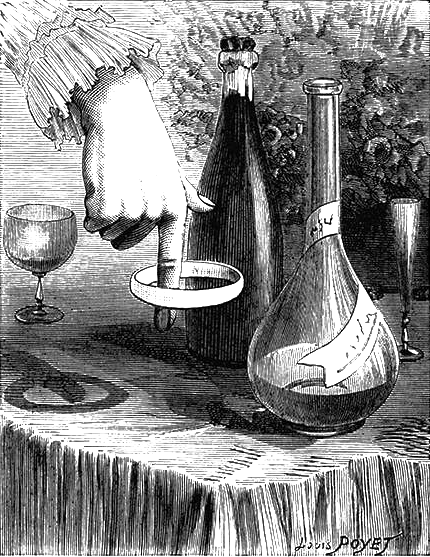
\includegraphics[width=45mm]{image/centforce.png}
\caption{centripetal force}
\end{figure}

\lipsum[9-14]

\chapter{Something}

\lettrine[lines=4]{E}{}\lipsum[14-23]

\chapter{Discussion}

\lettrine[lines=4]{M}{}\lipsum[24-31]

In this document some extra packages and parameters
were added. There is an encoding package
and pagesize and fontsize parameters.
In this document some extra packages and parameters
were added. There is an encoding package
and pagesize \autocite{Albarella2001} and fontsize parameters.

